\documentclass[a4paper,12pt]{report}
\usepackage[utf8]{inputenc}
\usepackage[T1]{fontenc}
\usepackage{lmodern}
\usepackage{mathtools}
\usepackage[catalan]{babel}
\usepackage{hyperref}
\usepackage{graphicx}
\usepackage{acronym}
\usepackage{eurosym}
\usepackage{pgfplots}
\usepackage[backend=biber]{biblatex}
\usepackage[auth-sc]{authblk}

\addbibresource{biblio/main.bib}

\date{}
\begin{document}

\acrodef{ia}[IA]{{inteligència artificial}}
\acrodef{ann}[ANN]{{xarxa neuronal artificial}}


\title{
	{\bf Filosofia del Software i Intel·ligència Artificial} \\
	Procediments
}
\author{
	Oriol Ventosa \and
	Marc Ferré \and
	Gonzalo Palacios \and
	Pol Gómez
}

\maketitle

\tableofcontents

\chapter{Introducció}
Els procediments del projecte de recerca es basen en la realització de diferents \emph{demos} (demostracions)
que tenen la intenció de oferir una introducció a les aplicacions de la \ac{ia}.

S'ha utilitzat el llenguatge de programació C++, i les llibreríes SFML \autocite{sfmllib} (per a gràfics) i FANN \cite{fannlib} (per a la
creació i entrenament de xarxes neuronals).

Les demos (junt amb el seu estat de progrés actual) són les següents:

\begin{itemize}
\item \emph{Demo 1} - joc de futbol sala (5 jugadors per equip), aprenentatje 'per esforç' (reinforcement) amb \ac{ann} evolutiva, estat inicial
\item \emph{Demo 2} - reconeixement de caràcters 0-9, \ac{ann}, estat avançat (ajustament de paràmetres d'aprenentatge, etc)
\item \emph{Demo 3} - conducció automàtica (circuit simple), reinforcement amb \ac{ann} evolutiva, estat inicial (físiques de conducció)
\item \emph{Demo 4} - ?
\end{itemize}

\emph{* La llista de demostracions pot variar fins a la versió final *}


\chapter{Xarxes Neuronals Artificials}
Les \emph{xarxes neuronals artificials} (ANN) són \emph{models computacionals 
inspirats pel sistema nerviós central dels animals (en particular, el cervell)} \autocite{nnpatrec}.

L'estructura d'una \ac{ann} és semblant a la d'un circuit electrònic: hi ha una capa o \emph{layer}
de $ q $ neurones d'entrada, o \emph{inputs}, i un layer de $ p $ neurones de sortida, o \emph{outputs}.
Això permet representar la seva estructura com si fos una funció matemàtica, $ f(x_0, x_1, ..., x_q) = \{y_0, y_1, ..., y_p\} $,
és a dir: un conjunt $ x $ d'entrades formen un conjunt $ y $ de sortides \ref{simple_ann}.

\begin{figure}[ht!]
\centering
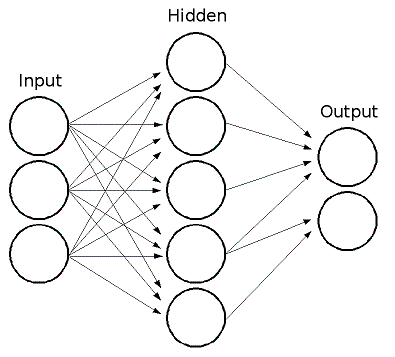
\includegraphics[width=80mm]{data/nn_simple.png}
\caption{El propòsit del layer \emph{hidden} s'explicarà més endavant.}
\label{simple_ann}
\end{figure}

La tasca principal d'una xarxa neuronal \emph{supervisada} és realitzar una \emph{aproximació de funció},
és a dir, a partir d'un seguit de valors de la funció (anomenat \emph{training set}), $ f(a) = b $, crear un model que s'ajusti a les dades
que se li ha subministrat \ref{func_approx}. Podríem, per exemple, entrenar una \ac{ann} per a que realitzés
una aproximació de la funció $ sin(x)$, però és més interessant entrenar-la amb objectius més sofisticats; tot
problema determinista que es pugui reduir a \emph{produir unes sortides a partir d'uns valors d'entrada}, es pot
solucionar, molt probablement, amb una xarxa neuronal.

\begin{itemize}
\item \emph{Conduir un cotxe:} la posició, la velocitat, els cotxes adjacents, la carretera... una gran quantitat d'entrades. La nova direcció, 
accelerar o frenar, com a sortides.
\item \emph{Predir el flux del mercat de valors:} la pendent de la gràfica del valor d'una acció, els últims moviments, els últims compradors...
la xarxa s'ha entrenat amb dades històriques, i l'historia es repeteix. El moviment de l'accionista com a sortida.
\item \emph{Reconèixer caràcters:} aquesta és la nostra parada per a continuar amb l'explicació de les \ac{ann}. El conjunt de píxels que formen 
l'imatge d'un caràcter com a entrades, i el número que representen els píxels com a sortida. És un exemple fàcil d'aplicar i enriquidor.
\end{itemize}

\begin{figure}[ht!]
\centering
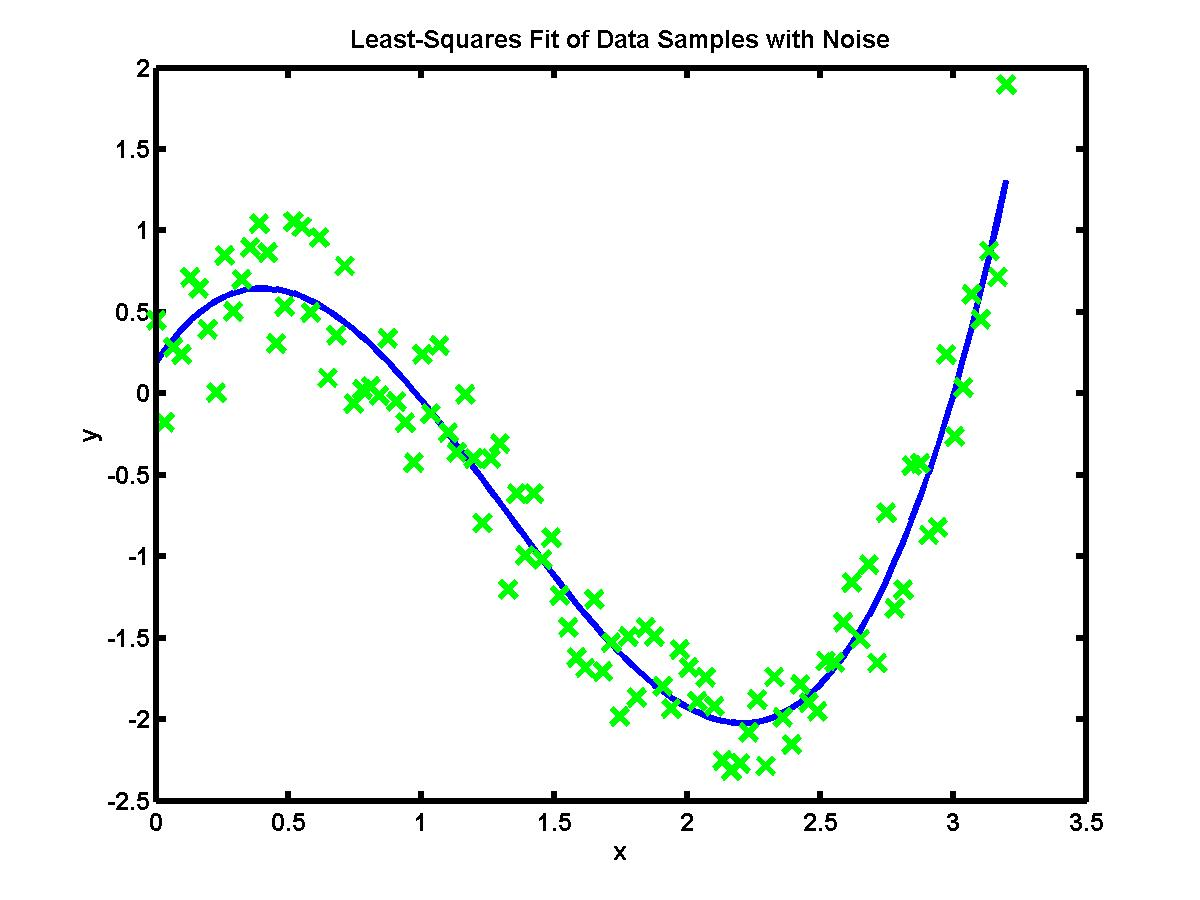
\includegraphics[width=80mm]{data/func_approx.jpg}
\caption{Exemple d'aproximació de funció. Els punts verds són els valors subministrats, el training set,
i la línia blava la funció que s'ha aproximat.}
\label{func_approx}
\end{figure}

\printbibliography

\end{document}
